\uuid{LA0L}
\exo7id{7744}
\titre{exo7 7744}
\auteur{mourougane}
\organisation{exo7}
\datecreate{2021-08-11}
\isIndication{false}
\isCorrection{true}
\chapitre{Géométrie projective}
\sousChapitre{Géométrie projective}
\module{Algèbre et géométrie}
\niveau{L3}
\difficulte{}

\contenu{
\texte{

}
\begin{enumerate}
    \item \question{Etant données les images $A'=h(A)$, $B'=h(B)$, $C'=h(C)$, et $D'=h(D)$ par une homographie $h$ de $P^2(\Rr)$ dans lui-même, construire à la règle les images des autres points.
    On indiquera l'ordre dans lequel les constructions sont effectuées.}
\reponse{~
    
    \begin{center}
        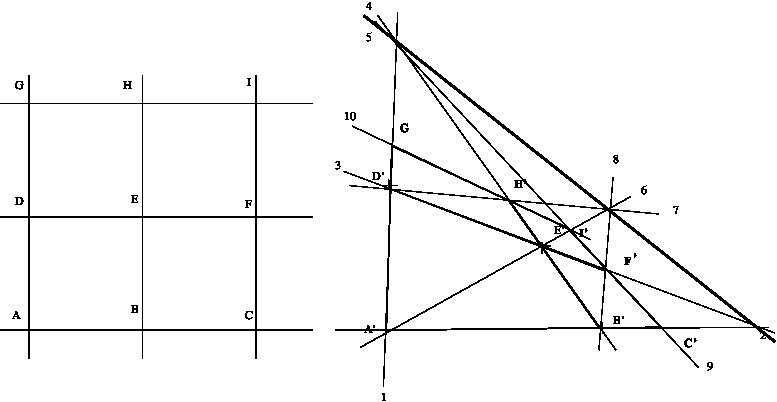
\includegraphics[scale=0.5]{images/LA0L-1}
    \end{center}}
    \item \question{Suffirait-il de connaître les images $A'=h(A)$, $B'=h(B)$ et $C'=h(C)$ ?}
\reponse{Non, il faut au moins avoir l'image d'un repère projectif.}
\end{enumerate}
}
